\section{Evaluation}
\label{sec:eval}
This section evaluates \meddle in terms of overhead, visibility into network traffic and 
the ability to map network traffic to the apps that generated it. We use the results in 
this section to inform the applications we build in \S\ref{sec:characterize-app} and \S\ref{sec:isp-behavior}.

\subsection{Methodology}
\label{sec:dataset}
Using \platname, we collected full packet traces from Internet activity generated by
mobile devices. We use this data to study how to map monitored traffic to applications, and to
analyze PII leakage. Below, we describe our data-collection methodology, which consists of
1) controlled experiments in a lab setting and 2) IRB-approved ``in the wild'' measurements 
gathered from real users during seven months.


\subsubsection{Controlled Experiments with Apps}
\label{sec:dataset-contr-exper}
Our goal with controlled experiments is 1) to obtain ground truth information 
about network flows generated by apps and devices, and 2) characterize the 
network activity for a large variety of apps in a lab setting. We use 
this data to understand how to model apps' network behavior, how to map network flows 
to the app that generated them and how to identify PII in those network flows. 

\noindent\textbf{Device setup.} We conducted our controlled experiments using two Android 
devices (running Android 4.0 and 4.2) and an iPhone running iOS 6. We start each set of controlled experiments
 with a factory reset of the device to ensure that software installed by previous 
 experiments cannot impact the network traffic generated by each device. 
 Then we connect the device to \platname{}  and begin
the experiment. 


\noindent\textbf{SSL bumping.} 
We use SSL bumping only in controlled experiments where \emph{no user traffic is intercepted}.
%, using a plugin to enable % SSL traffic decryption. 
We are also designing a study for IRB approval in which users can opt in to use SSL bumping for obfuscating PIIs in their SSL traffic.

\noindent\textbf{Manual tests.} We manually test the
100 most popular free Android apps in the \emph{Google Play} store and 209
iOS apps from the iOS App store on April 4, 2013. For each
app, we install it, enter user credentials %for the account 
if relevant, interact with it for up to 10 minutes, and uninstall
it. This allows us to characterize real user interactions with popular apps
in a controlled environment.  
We enter unique and distinguishable user credentials when 
interacting with apps to easily extract the corresponding PII from 
network flows (if they are not obfuscated). We use the same technique 
to test malware apps (\S\ref{subsec:malware}).

\noindent\textbf{Automated tests.} The second set of controlled experiments consist of fully-automated
experiments on 732 Android apps from a free,
third-party Android market, \emph{AppsApk.com}~\cite{appsapk}.
We perform this test because Android users can install
\emph{Third-party apps} without rooting their device. 
% that are not available on the
%\emph{Google Play} store, 

Our goal is to understand how these apps differ from those in the standard \emph{Google Play} 
store, as they are not subject to Google Play restrictions.
%\tbd{Is there different constraints on this free market, AR: They do not have paid application. All apps must be free.}
We automate experiments using \emph{adb} to
install each app, connect the device to the \meddle platform, and
start the app. Then we use \emph{Monkey}~\cite{adbmonkey}, an app-scripting 
tool, to perform a series of  approximately 100,000 actions that include
random swipes, touches, and text entries.  Finally, we use adb to
uninstall the app and reboot the device to forcibly end any
lingering connections. This set of experiments is limited to
Android devices because iOS does not provide equivalent 
scripting functionality. 
%\tbd{Are they stores from which you can download apps for non jail-broken iOS devices? DC: No.}

\subsubsection{In Situ Study}
\label{sec:dataset-wild-measurements}

The controlled experiments in the previous section provide us with 
ground-truth information for a large number of apps running in a controlled 
setting for a short period of time. To understand the network behavior of 
devices with real users ``in the wild'' over longer time periods, we conducted 
an IRB-approved measurement study with a small set of subjects, from 
Oct. 15, 2012 to Sep. 1, 2013.\footnote{The measurement study is ongoing, we report a subset of results.}

Our measurement data was collected from 26 devices: 10 iPhones, 4 iPads, 1 iPodTouch, and 11
Android phones.  The Android devices in this dataset include the
Nexus, Sony, Samsung, and Gsmart brands while the iPhone devices
include one iPhone~3GS, four iPhone~5, and five iPhone~4S.  These
devices belongs to 21 different users, volunteers for our IRB approved
study.  This dataset, called \mobWild, consists of 318 days with data; the number of 
days for each user varies from 5 to 315 with a median of 35 days.  For privacy reasons, the
SSL-Bumping plugin is \emph{disabled} for all measurements involving
real users.


\subsection{Overheads}
\noindent\emph{Network Latency.}
We first test indirection overhead from mobile networks to a \meddle instance. In the 
US with EC2, delays from mobile-network egress points to EC2 nodes are on generally less than 10\,ms. 
For other networks, we will achieve similarly low indirection overhead by placing instances in a cloud/hosting 
provider near subscribers and use DNS redirection (\eg via Amazon's Route 53) to direct clients to nearby instances. 

The other source of network delays is connection establishment time, incurred once per session. We measured 
50 VPN-connection establishment times on both iOS (iPhone 5 / iOS 6.1) and Android (Galaxy Nexus /
Android 4.2), for \wifi{} and cellular connections. We conduct tests in rapid succession to ensure the radio is in the high power state.
The \meddle server was running on a university network. 
For Android (using IKEv2), the maximum establishment time was 0.81 seconds on \wifi{} and 1.59 seconds on cellular. 
For iOS (using IKEv1), the connection takes longer due to the older protocol version: we observe a maximum of 2 seconds on \wifi{} and 2.18 seconds on cellular. 
Because each VPN session supports many flows, the amortized cost of connecting is  small. 
%\tbd{Cite results from latency to home gateways based on DSL results in PAM and IMC.}
%\tbd{Address comments in conext review on latency}

\noindent\emph{Power Consumption.}
Mobile devices expend additional power to establish, maintain and encrypt data for a VPN tunnel. 
To evaluate the impact on battery, we used a power meter to measure the draw from a Galaxy Nexus running Android 4.2. 
We run 10-minute experiments with and without the VPN enabled. 
For each experiment, we used an activity script that included Web and map searches, Facebook interaction, e-mail and video
streaming. 
The VPN leads to a 10\% power overhead. 
For iOS devices, we relied on the battery readings provided by iOS because we cannot attach a power meter directly to the battery.
We again found an approximately 10\% power overhead of using VPNs when we drained a fully charged battery while performing the operations performed during the tests for Android devices.  

%\item 
\noindent\emph{Traffic Volume.}
\meddle relies on IPsec for datagram encryption, thus there is an encapsulation overhead for each tunneled packet. 
To evaluate this overhead, we use 30 days of data from 25 devices that to compare encapsulated and raw packet sizes. 
We observe a maximum encapsulation overhead of 12.8\% (average approximately 10\%). 
For users that have limited data plans and consume most of their quota per month, this can have 
a significant impact. We note that this is partially offset by \meddle services such as content filtering and 
connection blocking. % and optimizations such as transcoding and compression. 

\noindent\emph{Scalability.} We currently use Amazon EC2 to support users at our cost. 
Without exploring opportunities for economies of scale, we estimate that 
it will cost less than a penny (\$0.0084) per user per day. At this cost, we can support up to 
10,000 users with research funds. If \meddle were to become extraordinarily popular, it would 
cost each user approximately a quarter per month to pay their own way. By comparison, 
data plans in the US tend to cost \$30-\$90 per month -- more than two orders of magnitude larger.

\subsection{Meddle Visiblity}

%We now highlight key features of the \mobWild dataset. 
We now use data gathered from users to demonstrate that there is a need for a platform like \meddle that provides a comprehensive view of Internet traffic from mobile devices. 
Note that due to the relatively small number of users in our study, we do not attempt to  
draw strong and generalizable conclusions. 

\noindent\textbf{Observation 1: \emph{End-host instrumentation provides a more complete view of 
Internet traffic from mobile devices.}} We infer the access technology (WiFi or cellular) for 
each session with the AS description from a \emph{WHOIS} lookup for each IP address used by a mobile device.
Based on this classification, the \mobWild dataset consists of traffic from 65 distinct ASes, of which 8 are cellular ASes and 7 are university networks.

We observe less diversity in cellular ASes compared to \wifi ASes.
During the measurement study, each device connected to our \platname server from at most two distinct cellular ASes. 
In contrast, a median of 4 \wifi ASes were observed per device and for one device we observed traffic from 36 different \wifi ASes spread across 5 countries.
In terms of traffic volumes, collectively our users with cellular connectivity transferred 24-56\% of their traffic over cellular and the remainder over WiFi. 
The key take-away is that, for the users in the \mobWild dataset, we would miss a large fraction of traffic generated by the mobile devices by instrumenting a single cellular carrier or WiFi access point. 
\meddle does not have this limitation.

\noindent\textbf{Observation 2: \emph{\meddle provides visibility into a wide range of traffic patterns}.} 
We use the classification provided by Bro~\cite{bro} to categorize flows as either TCP, UDP, or \emph{other}, along with subcategories HTTP, SSL and DNS.
Table~\ref{tab:summaryIOSAndroidTraffic} summarizes the traffic generated by user devices in our study. 

There are three key take-aways from this table. 
First, Web and SSL traffic dominate the traffic for users in the \mobWild dataset; 91.26\% (137.63 GB) of the traffic volume in the \mobWild dataset is either HTTP or SSL.
Second, there is significant diversity in the usage patterns for users with Android and iOS devices; the fraction of total flows over cellular or \wifi differ significantly for each OS. 
Third, a platform that cannot analyze SSL traffic will miss a large fraction of the traffic.
Indeed, a significant fraction of flows use SSL, which prevents classification using deep packet inspection.
This calls into question the overall effectiveness of traffic optimization approaches that rely on middlebox technologies that interpose on plaintext traffic (\eg page rewriting or downsampling media).
This motivates the need for a platform that not only covers multiple OSes and multiple access technologies but is also capable of intercepting all mobile Internet traffic, including SSL traffic, for the purpose of analysis and interposition. 

\begin{table}
\begin{small}
\begin{center}
\begin{tabular}{|p{0.11\columnwidth}|p{0.14\columnwidth}|r|r|r|r|}
\hline
{\bf IP} & \multirow{2}{*}{\bf Service} & \multicolumn{2}{|c|}{\bf Android} & \multicolumn{2}{|c|}{\bf iOS} \tabularnewline
\cline{3-6}
{\bf Protocol} &           &  \textbf{Cell.}  &  \textbf{\wifi}  &  \textbf{Cell.}  &  \textbf{\wifi}  \tabularnewline
\hline
\multirow{3}{*}{TCP}
       &  HTTP (\%)  & 44.83 & 68.23 & 60.07 & 76.92 \tabularnewline
\cline{2-6}
       &  SSL (\%)   & 44.74 & 20.89 & 36.19 & 14.11 \tabularnewline
\cline{2-6}
       &  other (\%) & 8.26  & 10.10  & 2.74  & 1.33 \tabularnewline
\hline
\multirow{2}{*}{UDP}
       &  DNS (\%)   & 1.31  & 0.58  & 0.64  & 0.38  \tabularnewline
\cline{2-6}
       &  other (\%) & 0.54  & 0.11  & 0.31  & 7.24  \tabularnewline
\hline
 Other &  other (\%) & 0.32  & 0.09 & 0.05  & 0.02  \tabularnewline
\hline
\multicolumn{2}{|c|}{\emph{total (\%)}} & 100.00 & 100.00 & 100.00 & 100.00 \tabularnewline
\hline
\multicolumn{2}{|c|}{\emph{Traffic Volume (GB)}}& 9.57 & 21.10 & 16.61  & 103.52 \tabularnewline
\hline
\multicolumn{2}{|c|}{\emph{\# Flows}}   & 927660 & 761735 & 730209 & 2796130 \tabularnewline
\hline
%\multicolumn{2}{|c|}{\emph{\# Devices}} & 10 & 11 & 10 & 15 \tabularnewline
%\hline
\end{tabular}
\end{center}
\end{small}
\caption{\textbf{Traffic volume (in percentage) of popular protocols and services on Android and iOS devices over cellular and \wifi.}
\emph{TCP flows are responsible for more than 90\% of traffic volume. Traffic share of SSL over cellular networks is more than twice the traffic share of SSL over \wifi.}} 
\label{tab:summaryIOSAndroidTraffic}
\end{table}


%\section{Data Analysis}
%
%In this section, we analyze the network traces gathered by \meddle to 
%1) provide summary statistics of data gathered from our 
%users ``in the wild'' and
%2) develop and evaluate several techniques for mapping network flows to 
%applications, which we will use in subsequent sections to identify privacy 
%leaks and malware.


%An important question for network characterization is which app is responsible for which 
%network flows. As we demonstrate in the following section, previous approaches are insufficient 
%for mapping the majority of apps to their corresponding network flows. We describe 
%several techniques to improve this mapping, and present results for controlled experiments 
%and the \mobWild dataset.

\subsection{Mapping Network Flows to Apps}
%\section{Traffic Classification}
\label{sec:classification-methodology}

Mapping network flows to apps is an important step for determining the origins of potentially costly 
network traffic, and for identifying which apps are responsible for privacy leaks. The following 
sections show that  \emph{previous approaches to mapping passively gathered traffic fail to identify
apps responsible for that traffic most of the time} and that \meddle facilitates a first look at 
determining which apps generate traffic over SSL connections.

%Previous work uses passively gathered data 
%to characterize such traffic, which can be useful for a variety of important topics that include 
%traffic engineering, optimization of network-enabled apps and understanding threats to user privacy. 


% 1) for the users in our study, traffic over WiFi and cellular networks 
%are qualitatively different, and studies that focus on only one technology will miss approximately 
%half of the traffic generated by devices; 

%\subsubsection{Classification of Mobile Apps and Services}

Table~\ref{tab:summaryIOSAndroidTraffic} suggests that apps, OS services, and libraries often rely on HTTP and SSL to exchange data.
%To analyze the behavior of mobile services we need to first associate the observed flows with the applications and the OS services responsible for the flows.
In the following analysis, we focus on identifying the apps, OS services, and other services responsible for these HTTP and SSL flows. 
We use ground-truth data from controlled experiments to show that the previous approach for classification fails 
for most popular apps; we then develop techniques to improve this mapping and apply it to our \mobWild dataset. 

\subsubsection{Improving HTTP Traffic Classification}
In \meddle, we need to know which app is responsible for Internet traffic using only network flow information. This section shows how to use \useragent and \httphost fields to identify the apps and services responsible for HTTP flows. Previous work~\cite{maier:mobtraffic,xu:appusage,falaki:mobileusage,falaki:smartphoneusage} is insufficient -- they use HTTP header fields to identify the \emph{category} of corresponding apps, not the specific app.


\begin{table} 
     \centering
     \begin{small}
     \begin{tabular}{|p{0.05\columnwidth}|p{0.08\columnwidth}|p{0.07\columnwidth}|p{0.08\columnwidth}|p{0.09\columnwidth}|p{0.09\columnwidth}|p{0.09\columnwidth}|p{0.09\columnwidth}|}
        \hline
        {\bf OS}&{\bf Store}&{\bf Apps}&{\bf Gen.}&\multicolumn{2}{|c|}{\bf Host} & {\bf User-}&{\bf Combi-} \tabularnewline
        \cline{5-6}    
             &        &     & {\bf HTTP} & {\bf App. } & {\bf Org.}& \bf{Agent}   & \bf{nation}  \tabularnewline                
        \hline    
        iOS  & Apple  & 209 & 176 & 83 (47.1\%)  &  119 (67.6\%)   &  149 (84.6\%)& 157 (89.2\%) \tabularnewline
        \hline
        And. & Google & 100 & 92  & 41 (44.5\%)  &  54 (58.6\%)    &  21 (22.8\%) &  59 (64.1\%)  \tabularnewline
        \hline    
        And. & Other  & 732 &  365 &  17 (4.6\%) &  79 (21.6\%)    &  52 (14.2\%)  & 83 (22.7\%)  \tabularnewline
        \hline
     \end{tabular}
     \end{small}
     \caption{\textbf{Classification of apps based on \httphost and \useragent.} \emph{ Most iOS apps use dedicated \useragent strings to fetch data over HTTP. A combination of \useragent and \httphost identifies the majority of Android and iOS apps.}}
     \label{tab:classification-success}
\vspace{\postfigspace}
\end{table}

%%
%% No HTTP Traffic from 209 - 38 = 171; 171 + 5 (OS possibly - confirm) = 176  ,
%% 181 unique signature, 7*2 = 14 duplicate (fooducate, fdct). 
%% 174 unique application signatures found
%% 5 UA belonged to OS services, geoservices, applecoremedia, gamedkit, securityd, mmsdk 
%% Ads from 98 - 4 -> 94 labels
%% Rough estimate of HTTP for apps because mapping  -- 414 files without HTTP
%%%
%% In amy dataset, 
%% 132 generate only ad traffic 


\noindent\textbf{Controlled experiments.}
In Table~\ref{tab:classification-success} we present results from our classification study using controlled experiments. To 
the best of our knowledge, we are the first to attempt to use ground-truth information to evaluate the 
effectiveness of app classification using only header data. 
%We begin classification using the \httphost field.

\emph{Classifying with \httphost:}
First, we note that 176 of the 209 iOS apps we manually tested generated HTTP traffic.
Column 5 of Tab.~\ref{tab:classification-success} shows that the \httphost field uniquely identified the corresponding app for 47\% of the iOS apps. 
Each app generated multiple flows, some of which did not contain the app signature in the \httphost field, \eg when contacting ad sites or CDNs. 
Such flows comprised 2\% to 85\% of the traffic volume from the iOS apps used during our measurements. 
The \httphost field also can identify the provider that released an app.
For example, we observed the name \emph{Zynga} in the \httphost field when using \emph{Farmville}, an app created by Zynga.
When testing an app, we noted down the name of its creator as the organization, and we searched this name in the \httphost field in the HTTP flows generated by this app.  
In column 6 of Table~\ref{tab:classification-success}, we see that classification by organization is effective for 67\% of iOS apps. 

We observe similar results for flows from apps in Google Play.
However, for the apps from the Third-party store we observe that the \httphost field is less effective. 
Primarily this is due to the fact that a majority of the apps we tested (about 77\%) were stand-alone services such as games. 
These apps contacted advertisement or or CDN sites that do not uniquely identify the app.
Along with the organizations of the apps we tested, we used the Google Play API~\cite{googleplay:api} to extract the names of the creators (organizations) for the 5000 most popular Android apps on the Google Play store. 

\emph{Classifying with \useragent:} 
We observed a non-empty \useragent string in more than 99.7\% of the HTTP flows from iOS and 90.9\%flows from Android. 
A \useragent string may contain an app identifier and other auxiliary information such as details of the OS~\cite{mozilla:useragentdetection}. 
For example, Yahoo Mail's \useragent string contains the string \emph{YahooMobileMail/1.0}. 
However, some apps use more generic \useragent strings such as \emph{AppleCoreMedia} (streaming video on iOS) or \emph{Dalvik} (generic text for Android). 
To extract the app information, we use regular expressions to filter the auxiliary information from the \useragent and cluster the extracted tokens using the edit distance.

Table~\ref{tab:classification-success} shows that 84.6\% of the 176 iOS apps generating HTTP traffic were correctly identified by their \useragent, which we verified by manual inspection.
In contrast, the \useragent was useful in identifying only 23\% of the Android apps generating HTTP traffic, meaning previous techniques depending solely on the \useragent will fail~\cite{maier:mobtraffic,xu:appusage}. 
For the 27 iOS apps which we failed to identify, we observed signatures for OS services and libraries.
Similarly, the majority of Android HTTP traffic contained flows with the default \useragent (\eg, \emph{Dalvik}).
%Further, for the apps from the third-party store, we observe that the \useragent for ads and analytics libraries such as \emph{Google Analytics} and \emph{Adsense for Mobile} were the most common \useragent after the default \useragent.
% such as \emph{Apple Core Media}, \emph{Game Kit}, \emph{Geo Services}, etc. and signatures of third-party libraries and services such as \emph{Google Analytics} and \emph{Adobe Air}.
%,falaki:mobileusage,falaki:smartphoneusage

\emph{Combination of \useragent and \httphost:} 
In Table~\ref{tab:classification-success}, we observe that the \useragent is more effective for mapping iOS apps while the \httphost is more effective for Android apps; however, neither alone is a complete solution. 
We therefore rely on a combination of \useragent and \httphost to classify HTTP traffic. 
For our classification, we first try to classify the HTTP flow using the \useragent.
We use the \httphost field only if we were unable to extract any useful signature from the \useragent field. 
In Table~\ref{tab:classification-success}, we observe that by using a combination of the \useragent and \httphost we were able to identify 64\% of the Android apps and 89\% of the iOS apps. 
%To fill this gap, we are currently investigating how to use ad-network identifiers to classify apps. 

% \begin{figure}
% \subfloat[iOS]{\label{fig:http-wordcloud-ios}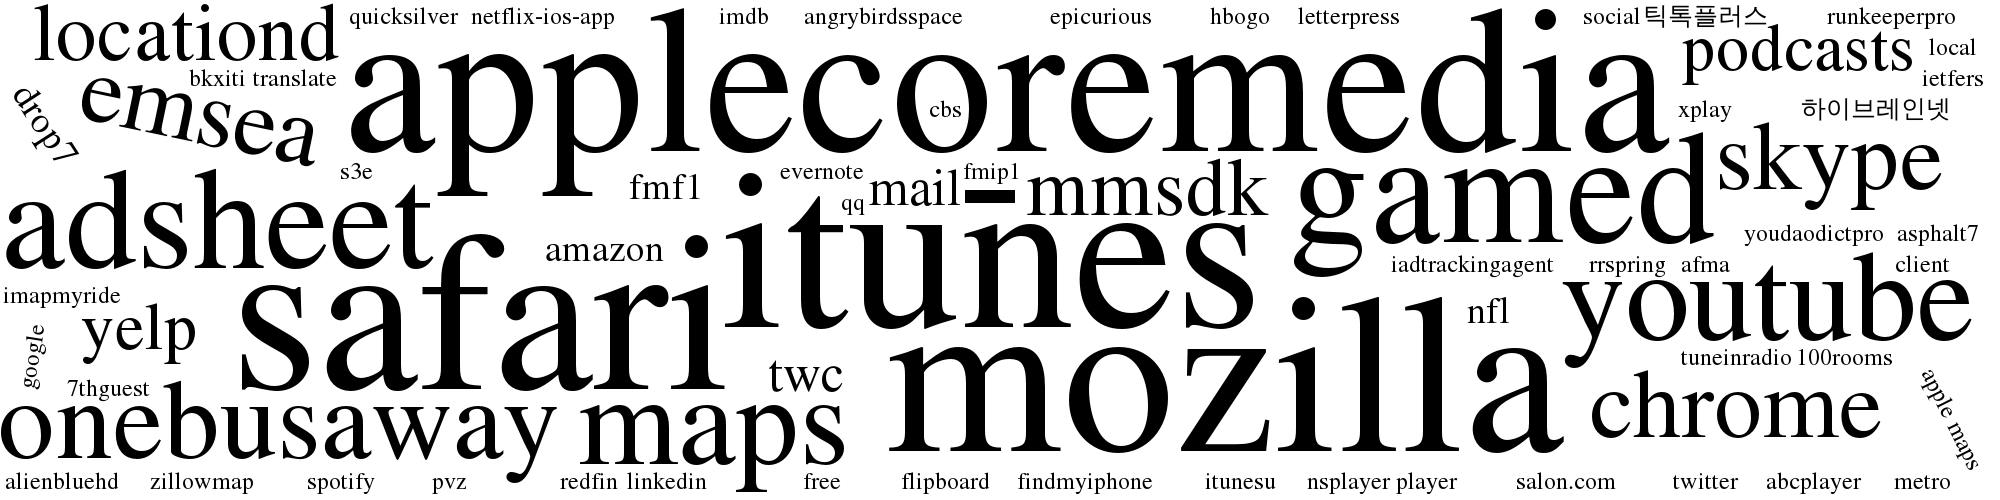
\includegraphics[width=\columnwidth]{figures/wordcloud_useragentsignature_ios_image.png}}\newline
% \subfloat[Android]{\label{fig:http-wordcloud-android}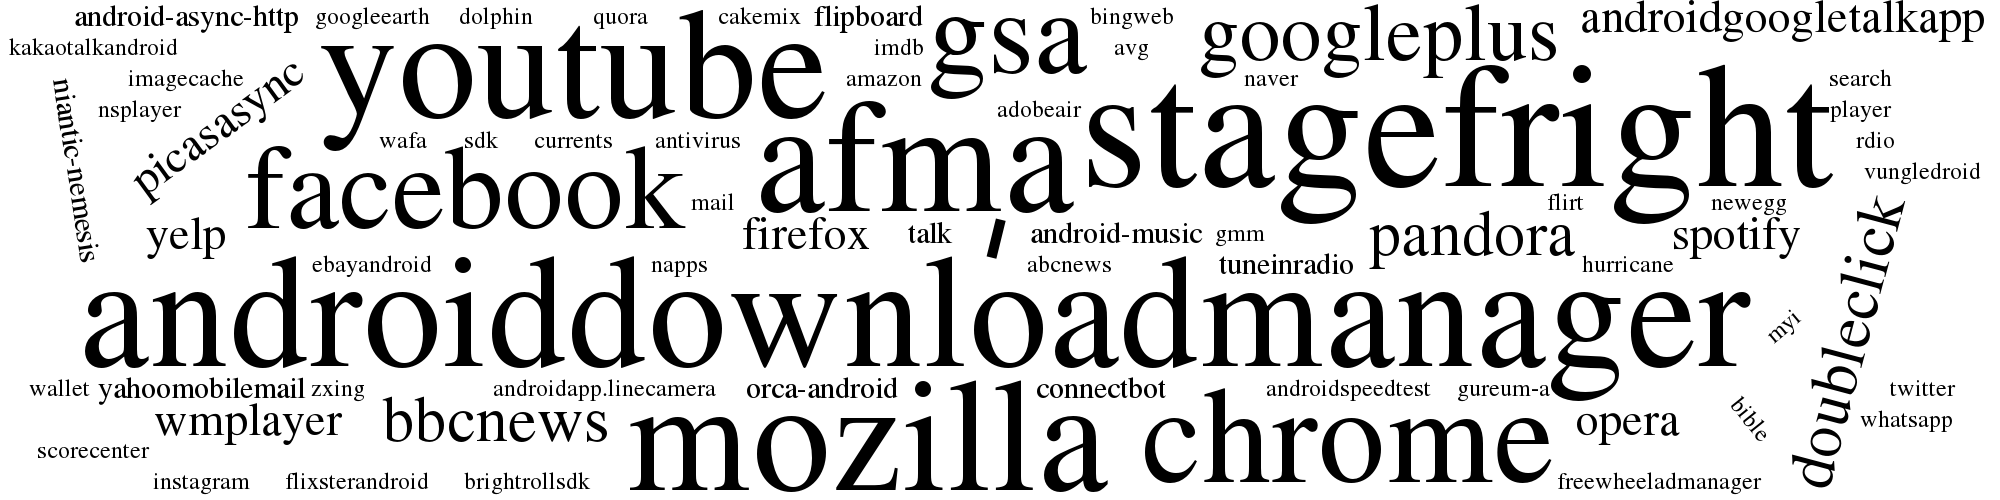
\includegraphics[width=\columnwidth]{figures/wordcloud_useragentsignature_android_image.png}}
% \caption{\textbf{\useragent signatures in  iOS and Android HTTP flows.} \emph{The font weight represents the number of users for which a particular signature was observed.}}
% \vspace{\postfigspace}
% \label{fig:http-wordcloud}
% \end{figure}

%We now describe the results of classifying HTTP traffic in the \mobWild dataset. %mapping data gathered from our user study.
%Using only the \useragent on the \mobWild dataset, we were able to identify 256 iOS and 86 Android apps, OS libraries, and services. 
%The \emph{word cloud} in Fig.~\ref{fig:http-wordcloud} contains the summary of our results; the font size of an app/service name is proportional to the number of users for which it was observed.
%Note that \emph{Apple Core Media} and \emph{Stagefright} are services for downloading media content on iOS and Android devices, respectively.
%For the iOS devices in the \mobWild dataset, we observe a signature of \emph{Apple Core Media} in more than 98.45\% of the content downloaded from the YouTube servers (identified by their \httphost field).
%Similarly, we observe that YouTube flows contain ``Stagefright'' in HTTP headers. % to Android devices depending on the OS version. 
%We observe a similar signatures for other popular media services such as Netflix, YouTube, Vimeo, Pandora, etc, so we use the \httphost field to identify these Web services.
%\drc{AM: Suggests removing word cloud. PG doesn't like them either.}

\begin{table}
\centering
\begin{small}
\begin{tabular}{|p{0.15\columnwidth}|p{0.2\columnwidth}|c|c|c|c|}
\hline
\multirow{2}{*}{\bf Technique}&\multirow{2}{*}{\bf Category} & \multicolumn{2}{c|}{\bf iOS} &  \multicolumn{2}{c|}{\bf Android} \tabularnewline
\cline{3-6}
&   & {\bf Bytes}  & {\bf Flows} & {\bf Bytes} & {\bf Flows}   \tabularnewline
&   & {\bf (\%)}  & {\bf (\%)} & {\bf (\%)} & {\bf (\%)}   \tabularnewline

\hline
\multirow{2}{*}{\useragent} &Apps             & 43.21  & 85.73 & 15.01 & 75.17 \tabularnewline
\cline{2-6}
                            & OS Services$^{*}$            &  0.19  & 3.82 & 17.42 & 0.81 \tabularnewline
\hline
\useragent + &Media (Popular)         & 51.36  & 7.12  & 61.98 & 3.56 \tabularnewline
\cline{2-6}
\httphost  &Media (Other)           & 4.90  &  0.85 &  0.68 &  0.12 \tabularnewline
\hline
\httphost & Other Apps/Web-services  & $<$0.01 & 0.49 & 1.53  & 12.98 \tabularnewline
\hline
\multicolumn{2}{|c|}{Total Classified}  & {\bf 99.6} & {\bf 98.01} & {\bf 96.62} & {\bf 92.64} \tabularnewline
\hline
\end{tabular}
\end{small}
\caption{\textbf{Effectiveness of mapping HTTP traffic}. \emph{OS services$^{*}$ includes services other than those used to download media content.}}
\label{tab:classify-http}
\end{table}

\textbf{In situ data.}
Table~\ref{tab:classify-http} shows that a combination of \useragent and \httphost field in HTTP headers can map more than 92\% of the traffic (flows and bytes) from iOS and Android devices.
Using only the \useragent on the \mobWild dataset, we were able to identify 256 iOS and 86 Android apps, OS libraries, and services. 
We observe that the \useragent is more effective in identifying iOS apps compared to Android apps, which concurs with what we observed during our controlled experiments, 
We observe that media from popular hosts in our \mobWild dataset, including Netflix, YouTube, Pandora, Spotify, and Vimeo, contribute to more than 50\% of the traffic volume from iOS and Android devices.
We also observe that unmapped media served from CDNs and others hosts comprises less than 5\% of the traffic volume for the iOS and Android devices. 

To summarize, by using a combination of \useragent and \httphost we were able to classify more than 92\% of the iOS and Android traffic by flows and bytes. 
%\drc{From PG: How is mapping to organization done?}

\subsubsection{SSL Traffic Mapping without Decryption}

SSL flows provide limited information in plaintext to identify apps. 
For the traces captured during our controlled experiments, we use SSL bumping to map HTTP flows using the techniques described in the previous section. 
However, we did not perform SSL bumping for the devices in the \mobWild dataset, so we now describe how to 
map SSL flows \emph{without decryption}. 

\noindent\textbf{Overview of mapping technique.}
Using port numbers, we observe in that more than 98\% of SSL flows observed in our controlled experiments were due to HTTPS, the rest of the flows were due to email, instant messaging, and OS notification services. 
We therefore focus our attention on identifying the apps responsible for the HTTPS flows.
We use DNS responses and subsequent SSL handshakes to determine the \emph{hostnames} of the remote hosts contacted by mobile devices.
After identifying hostnames, we map them to apps using the technique described in the previous section.

%During manual examination of the results, we observe that Google and Apple to the be two main groups of organizations: Google and Apple.

% After identifying a hostname, we map the corresponding traffic in two phases.
% In the first phase we use the port number and hostname to identify the service 
% and group the traffic based on service. \drc{Why are you using the term ``service'' instead of app? 
% Why is this classification so different from the previous section? Need to make it more uniform.}
% The five most popular groups that we found in our dataset are social network, mail, media, instant messages, and notification.
% For example, flows to \url{facebook.com}, \url{twitter.com}, \url{plus.google.com} are grouped as social networks.
% Traffic to well known email ports such as TCP port 993, and traffic to hosts such as \url{mail.google.com} are classified as mail traffic.
% Similarly, we use documented ports to identify notification services (Android push) and instant messages (Facebook Messenger).

% In the second phase, we group hostnames that do not contain details of Web services.
% For example, the hostname \url{fbcdn-photos-a.akamaihd.net} indicates that the traffic is due to Facebook (due to \emph{fbcdn}), while \url{www.googleapis.com} hides the underlying app.
% We group hostnames that hide the app and Web service based on the parent organization.
% During manual examination of the traces, we observe two main groups: Google Services and Apple Services.
% Google Services includes flows whose remote hosts are served by Google, \eg \url{www.googleapis.com}, while Apple Services includes flows to servers managed by Apple, \eg \url{*.phobos.apple.com}
% This mapping, though crude, gives insights on the key sources of SSL traffic.

\noindent\textbf{Identifying hostname using the SSL Handshake.}
We first use the common name (CN) field of certificates to identify the servers that exchanged data using HTTPS.
We observe that less than 25\% of the HTTPS traffic from iOS and Android contains the fully qualified domain name (FQDN) in the subject of the certificate; the rest of the traffic either contains regular expressions such as *.google.com or is a continuation of a previous SSL session. 
To further resolve the hostnames, we rely on the \emph{Server Name Indication} (SNI) used by SSL flows~\cite{rfc:servernametls}.
Servers that host multiple services use the SNI to distinguish these services.   
For example, we observe an SNI of \url{plus.google.com} and \url{s.youtube.com} in two flows that used a certificate with a CN \url{*.google.com}.
Using either the certificate or the SNI we identified the hostname for	 less than 40\% of HTTPS traffic.

\noindent\textbf{Identifying hostname using the DNS messages.} 
For the remaining flows we use DNS messages exchanged by the mobile device with its DNS server before starting the HTTPS flows, a technique similar to DN-Hunter~\cite{bermudez:dnhunter}.
DN-Hunter relies on the most recent FQDN that corresponds to the IP address, however in our controlled experiments we observe Android and iOS devices use the first entry in DNS response while resolving hostnames.
We therefore use the latest DNS response that contains the IP address of the Web service in the first position.
In spite of the potential usefulness of DNS responses, we give a high priority to the SNI and the certificates because the DNS response differs from these in 9.2\% of the iOS traffic and 5.6\% of Android traffic.
This difference is due to caching of DNS responses by the apps.

% \begin{table}
% \centering
% \begin{small}
% \begin{tabular}{|p{0.1\columnwidth}|p{0.2\columnwidth}|c|c|c|c|}
% \hline
% \multirow{2}{*}{\bf Phase} & \multirow{2}{*}{\bf Category} & \multicolumn{2}{c|}{\bf iOS Traffic} &  \multicolumn{2}{c|}{\bf Android Traffic} \tabularnewline
% \cline{3-6}
%  &         & {\bf Bytes}  & {\bf Flows} & {\bf Bytes} & {\bf Flows}   \tabularnewline
%  &         & {\bf (\%)}  & {\bf (\%)} & {\bf (\%)} & {\bf (\%)}   \tabularnewline
% \hline
% \multirow{5}{*}{Apps (A)}
% & Social Ntwks    & 12.81 &  7.74 & 35.39 & 19.28 \tabularnewline
% \cline{2-6}
% & Mail               &  6.11 &  9.26 &  6.46 & 11.02 \tabularnewline
% \cline{2-6}
% & Media              &  0.94 &  0.25 &  3.66 &  3.62 \tabularnewline
% \cline{2-6}
% & Instant Msg   &  3.70 & 14.09 &  0.21 &  0.48 \tabularnewline
% \cline{2-6}
% & Notifications     &  4.69 & 17.45 &  2.02 &  6.57 \tabularnewline
% \cline{2-6}
% %\hline
% & \emph{Total (A) }       & {\em 28.25} & {\em 48.79} & {\em 47.74} & {\em 40.97} \tabularnewline
% \hline
% \multirow{2}{*}{Organization (B)}
%  & Google Svcs   & 36.32 & 17.56 & 47.31 & 48.27 \tabularnewline
% \cline{2-6}
%  & Apple Svcs    & 25.26 & 28.26 & $<$0.01 & $<$0.01 \tabularnewline
% \cline{2-6}
% \cline{2-6}
% & \emph{Total (B) }       & {\em 61.58} & {\em 45.82} & {\em 47.31} & {\em 48.27} \tabularnewline
% \hline
% \multicolumn{2}{|c|}{\emph{Total (A + B)}}       & {\em \bf 89.83} & {\em\bf 94.61} & {\em\bf  96.10}  &  {\em\bf  89.24} \tabularnewline
% \hline
% \end{tabular}
% \end{small}
% \caption{\textbf{Mapping SSL traffic in the \mobWild dataset.} \emph{The iOS and Android SSL traffic in the \mobWild dataset is dominated by Google and Apple Services. The share of Social Network traffic is higher for Android devices because the default photo backup services on Android devices uses the Google Plus (and Picasa) Social Network.}}
% \label{tab:classify-ssl-traffic}
% \end{table}



\begin{table}
\centering
\begin{small}
\begin{tabular}{|p{0.3\columnwidth}|c|c|c|c|}
\hline
\multirow{2}{*}{\bf App/Org} & \multicolumn{2}{c|}{\bf iOS Traffic} &  \multicolumn{2}{c|}{\bf Android Traffic} \tabularnewline
\cline{2-5}
                              & {\bf Bytes}  & {\bf Flows} & {\bf Bytes} & {\bf Flows}   \tabularnewline
                              & {\bf (\%)}  & {\bf (\%)} & {\bf (\%)} & {\bf (\%)}   \tabularnewline
\hline

Apps            & 28.25 & 48.79 & 47.74 & 40.97 \tabularnewline
\hline
Google Services & 36.32 & 17.56 & 47.31 & 48.27 \tabularnewline
\hline
Apple Services  & 25.26 & 28.26 & $<$0.01 & $<$0.01 \tabularnewline
\hline
{\emph{Total}}  & {\em \bf 89.83} & {\em\bf 94.61} & {\em\bf  96.10}  &  {\em\bf  89.24} \tabularnewline
\hline
\end{tabular}
\end{small}
\caption{\textbf{Mapping SSL traffic in the \mobWild dataset.} \emph{The SSL traffic from the iOS and Android devices in the \mobWild dataset is dominated by Google and Apple services.}}
\label{tab:classify-ssl-traffic}
\end{table}

\noindent\textbf{Mapping results.} 
Table~\ref{tab:classify-ssl-traffic} shows our SSL mapping results on the SSL traffic in the \mobWild dataset. 
We first group hostnames to the apps and we were able to identify the apps for more than 40\% of the iOS and Android SSL flows.
For flows whose hostnames are ambiguous, we group them according to organizations.
During manual examination of the results, we observe that Google and Apple to be the two main organizations that contributed to the majority of the flows; we label these flows as Google Services and Apple Services. 

In Table~\ref{tab:classify-ssl-traffic}, we observe that 61.5\% of iOS and 47.3\% of Android traffic (by bytes) is respectively 
to Google and Apple servers where the hostname does not contain signatures of the app.
This share does not include the traffic to Google and Apple servers that we classified as apps.
For example, flows to \url{mail.google.com} were classified as GMail and are placed in the category apps, while flows to \url{www.googleapis.com} is categorized as Google Services. 
Google services and Apple services are therefore the largest sources of SSL traffic in our \mobWild dataset.

In summary, using the certificates, SNI, and DNS messages, we were able to identify the hostname of the remote hosts for more than 89\% of the SSL flows.
We observe that Google and Apple are the dominant sources of SSL traffic for the Android and iOS devices in the \mobWild dataset.

\subsubsection{Summary}

We use the a combination of \useragent and \httphost field to identify apps responsible for HTTP flows.
On applying our technique to the \mobWild dataset, we were able to classify more than 92\% of the iOS and Android traffic by flows and bytes. 
We observe that the \useragent field is more effective to identify HTTP flows from iOS devices compared to Android devices.
We speculate that this behavior is because of the strict coding practices mandated by Apple while packaging iOS apps~\cite{xcode:distrib}.

We use certificates, SNI, and DNS messages to map SSL flows, and we were able to classify more than 90\% of SSL traffic in the \mobWild dataset using our classification technique. 
To the best of our knowledge, we are the first to study the effectiveness of these fields in classifying SSL flows from mobile devices.

%%% Local Variables: 
%%% mode: latex
%%% TeX-master: "main"
%%% End: 


